\chapter{Аналитический раздел}
\label{cha:analysis}
	Перед проведением анализа необходимо разбить реализацию на независимые части. Для каждой предстоит выбрать алгоритм, удовлетворяющий поставленным задачам. Проанализировав возможные методы реализации были выделены следующие подсистемы:
\begin{itemize}
\item Способы управления курсором.
\item Передача данных с Android-устройства.
\item Обработка полученных данных.
\item Взаимодействие с ядром.
\end{itemize}
\begin{figure}
  \centering
  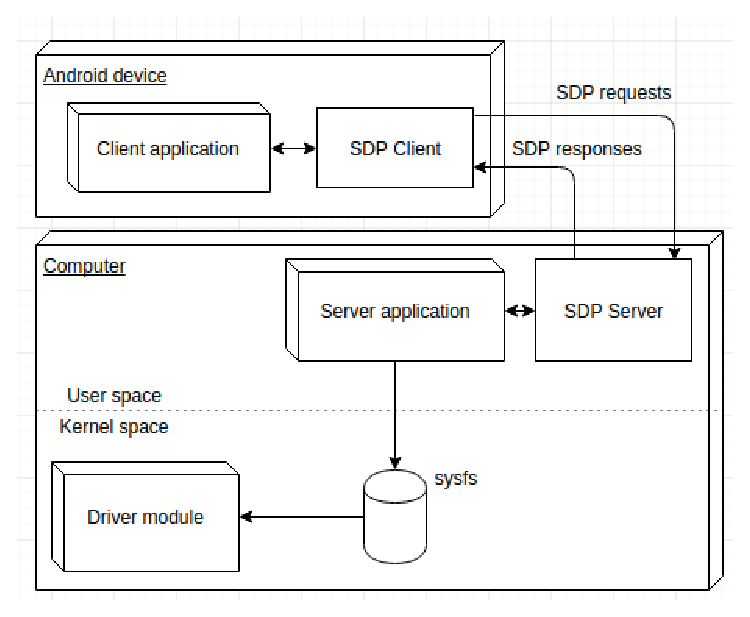
\includegraphics[scale=0.75]{analysis/structure}
  \caption{Общая структура.}
  \label{fig: view_arch}
\end{figure}
\label{sec: gyro&accel}
\section{Выбор способа управления}
	Для выбора способа управления необходимо отталкиваться от поставленных задач. Самый распространенный вариант - имитация сенсорной панели. При такой реализации дрожание курсора зависит лишь от задержки обработки данных. С другой стороны, присутствие в Android-устройствах таких датчиков\cite{gyr&accel}, как G-сенсор и гироскоп, дают дополнительную степень свободы, что позволяет получить большую функциональность.
	
	Гироскоп (гиродатчик) - устройство, позволяющее определить ориентацию в пространстве, используя гравитацию Земли. По количеству степеней свободы различают: двухстепенные и трехстепенные. На Android устройствах на сегодняшний день установлены вибрачионные микрогироскопы, принцип действия которых основан на силе Кориолиса\cite{coriolis}. 
	
	Акселерометр (G-сенсор) - устройство, предназначенное для измерения негравитационного ускорения. Различают три типа: однокомпонентные, двухкомпонентные и трехкомпонентные. Чтобы определить ориентацию в пространстве, необходимо данные измерения проинтегрировать, получая инерциальную скорость и координаты устройства. 

	Основным из преимуществ гироскопа является то, что акселерометр не в состоянии отличить гравитационное ускорение от любого другого. Находясь в системе отсчета, которая ускорено движется в определенном направлении, данный датчик будет показывать некорректные результаты. Гироскопы в свою очередь ориентируются лишь на гравитацию и не зависят от внешних факторов, поэтому и были выбраны в качестве способа управления.
\label{sec: bt&wifi}
\section{Методы передачи данных}
	Взаимодействие Android-устройства и персонального компьютера является необходимой частью реализации, поэтому необходимо выбрать один из существующих методов. Основными факторами выбора будут: радиус действия, скорость передачи и сложность настройки. Вариант с USB 3.0, не смотря на высокую скорость, не подходит из-за наличия проводной передачи данных.
	
	Bluetooth и wi-fi\cite{bt&wifi} являются беспроводными стандартами связи и используют для передачи данных определенные радиочастоты. Чтобы определиться с выбором метода, составим таблицу из самых распространенных стандартов с данными о радиусах действия и максимальных скоростях передач.
\begin{center}
\begin{table}[h]
  \caption{Сравнение стандартов}
  \begin{tabular}{|r|c|c|}
 	\hline
    Стандарт 		& Дистанция(в помещении), m & Скорость, Mbps \\
    \hline
    Wi-fi			&                	 		&              	 \\
    \hline
	IEEE 802.11.g   & 			38 		   		&    	54     	 \\
    IEEE 802.11.n   & 			70		   		&      600     	 \\
    \hline
    Bluetooth		&					   		&				 \\
    \hline
    Bluetooth 3.0	&			10		   		&		24		 \\
    Bluetooth 4.0	&			60	 	   		&		30 		 \\
    \hline
  \end{tabular}
  \label{tabl: bt&wifi}
\end{table}
\end{center}

	В таблице~\ref{tabl: bt&wifi} наглядно видно, что wi-fi обладает лучшими характеристиками. Но для передачи информации он требует тщательной настройки параметров, а также обязательного наличия третьего звена - точки-маршрутизатора. Возможен вариант соединения ad-hoc, который позволяет соединяться напрямую, но при этом станет невозможно подключить другие устройства. Bluetooth же не требует никакого дополнительного конфигурирования и позволяет подключить несколько устройств одновременно. Для передачи координат с Android-устройства хватает скорости передачи и bluetooth, поэтому он выбран для реализации передачи информации.

\label{sec: int_event}	
\section{Интерфейсы событий}
	В операционной системе Linux для решения поставленной задачи существует специальная подсистема ввода ядра\cite{ldd3}, которая объединяет все рассеянные драйвера для обработки перифирийных устройств. Одним из ее плюсов является удобный интерфейс событий, позволяющий драйверу не создавать и не управлять узлами /dev и связанными с ними методами доступа. Вместо этого он имеет возможность вызывать API для ввода, чтобы отправить движения мыши. Такие системы, как X Window, хорошо взаимодействуют с интерфейсами событий, экспортируемыми подсистемой ввода. 

	Чтобы выбрать один из возможных интерфейсов, необходимо обозначить требования, которым он должен соответствовать, и ознакомиться со всеми доступными вариантами. Исходя из задач, поставленных в рамках реализации, основным требованием к интерфейсу является необходимая функциональность. Кроме движения мыши, драйвер событий должен предоставлять возможность нажатия на кнопки мыши. Рассмотрим три возможных варианта: evdev, mousedev и собственный интерфейс.
	
\paragraph{Интерфейс evdev}

	<<\verb|Evdev|>> - универсальный драйвер событий ввода. Каждый пакет события, создаваемый <<\verb|evdev|>>, имеет строго определенный формат и содержит в себе следующие параметры: время, тип события, код события, значение события. Одно из преимуществ интерфейса - тесное взаимодействие с драйвером устройством для X Window, которые используются во всех UNIX-подобных ОС. Благодаря этому факту, данный драйвер событий является простым в использовании и универсальным. Набор функционала интерфейса сопоставим минимально требуемому для решения поставленной задачи.
	
\paragraph{Интерфейс mousedev}

	<<\verb|Mousedev|>> - специальный драйвер событий ввода для мыши. Имеет стандартный набор точек входа: подключение устройства, отсоединение устройства, открытие, закрытие, чтение и запись файла устройства. В отличие от универсального evdev, этот интерфейс предназначен лишь для одного перефирийного устройства. В драйвере реализуются события следующих типов:
\begin{itemize}
\item \texttt{EV\_ABS} - код события, связанного с абсолютным изменением значений координат по осям.
\item \texttt{EV\_REL} - код события, связанного с относительным изменением значений координат по осям.
\item \texttt{EV\_KEY} - код события, связанного с нажатием кнопки.
\item \texttt{EV\_SYN} - описывает разделенные во времени или пространстве события (для multitouch сенсоров).
\end{itemize}

	Отличительной особенностью является событие EV\_SYN, позволяющая взаимодействовать писать драйвера устройства для сенсорных панелей.
	
\paragraph{Интерфейс mydev}

	Помимо готовых вариантов, имеется возможность написать собственный драйвер событий. Чтобы его написать, требуется экспортировать его в пользовательское пространство с помощью \texttt{/dev/input/mydev}, создать структуру, которая хранит в себе следующие данные:
\begin{itemize}
\item Обработчик сообщений о событиях, посылаемых драйверами устройств ввода.
\item Указатель на методы управления, находящиеся в \texttt{/dev/input/mydev}.
\item Младший номер \texttt{/dev/input/mydev}.
\item Имя драйвера событий.
\item Функцию регистрации драйвера.
\item Функцию отмены регистрации драйвера.
\end{itemize} 

	Является более гибким вариантом, чем два, представленных выше, поскольку мы сможем постепенно наращивать функционал драйвера событий.
	
\paragraph{Итоговый выбор}

	Для решения поставленной задачи целесообразней использовать универсальный драйвер событий ввода. Поскольку он оснащен требуемой функциональностью, и прост в использовании.
	
%%% Local Variables: debug
%%% mode: latex
%%% TeX-master: "rpz-os"
%%% End: